% This must be in the first 5 lines to tell arXiv to use pdfLaTeX, which is strongly recommended.
%\pdfoutput=1
% In particular, the hyperref package requires pdfLaTeX in order to break URLs across lines.

\documentclass[11pt]{article}

% Remove the "review" option to generate the final version.
% \usepackage[review]{acl}
\usepackage{acl}

% Standard package includes
\usepackage{times}
\usepackage{latexsym}

% For proper rendering and hyphenation of words containing Latin characters (including in bib files)
\usepackage[T1]{fontenc}
% For Vietnamese characters
% \usepackage[T5]{fontenc}
% See https://www.latex-project.org/help/documentation/encguide.pdf for other character sets

% This assumes your files are encoded as UTF8
\usepackage[utf8]{inputenc}

% This is not strictly necessary, and may be commented out,
% but it will improve the layout of the manuscript,
% and will typically save some space.
\usepackage{microtype}

% If the title and author information does not fit in the area allocated, uncomment the following
%
%\setlength\titlebox{<dim>}
%
% and set <dim> to something 5cm or larger.

\usepackage{graphicx}

\title{Referring as a collaborative process: learning to ground \\ language through language games} % Discriminating 3D-objects using
% Author information can be set in various styles:
% For several authors from the same institution:
% \author{Author 1 \and ... \and Author n \\
%         Address line \\ ... \\ Address line}
% if the names do not fit well on one line use
%         Author 1 \\ {\bf Author 2} \\ ... \\ {\bf Author n} \\
% For authors from different institutions:
% \author{Author 1 \\ Address line \\  ... \\ Address line
%         \And  ... \And
%         Author n \\ Address line \\ ... \\ Address line}
% To start a seperate ``row'' of authors use \AND, as in
% \author{Author 1 \\ Address line \\  ... \\ Address line
%         \AND
%         Author 2 \\ Address line \\ ... \\ Address line \And
%         Author 3 \\ Address line \\ ... \\ Address line}

\author{Dominik Künkele$^{1}$ \and Simon Dobnik$^{1,2}$ \\
        Department of Philosophy, Linguistics and Theory of Science$^{1}$ \\ 
        Centre for Linguistic Theory and Studies in Probability (CLASP)$^{2}$ \\
        University of Gothenburg, Sweden \\
        \texttt{dominik.kuenkele@outlook.com} \and \texttt{simon.dobnik@gu.se}}

% \author{Dominik Künkele \\
%   Affiliation / Address line 1 \\
%   Affiliation / Address line 2 \\
%   Affiliation / Address line 3 \\
%   \texttt{dominik.kuenkele@outlook.com} \\\And
%   Simon Dobnik \\
%   Affiliation / Address line 1 \\
%   Affiliation / Address line 2 \\
%   Affiliation / Address line 3 \\
%   \texttt{simon.dobnik@gu.se} \\}

\begin{document}
\maketitle
\begin{abstract}
  How do artificial agents based on neural networks coordinate on a new language through referential games over 3-dimensional scenes?
  We extended a popular CLEVR dataset to control for different combinations of features of target and distractor objects and examine the success of referential grounding learned by the agents.
\end{abstract}

\section{Introduction}
% TODO:
% \begin{itemize}
%   \item how can models reidentify attributes (and objects) from learned encodings in an artificial language \textbf{(done)}
%   \end{itemize}

Agents interact with the physical world through their action and perception and with other agents through language.
Their sensors and actuators % (if they are artificial agents, but the same also holds for natural agents)
allow them to sample the world and their own state using measures that are continuous in nature such as intensity of light, distance, angles, velocity and others which can be measured with a high degree of accuracy.
On the other hand language that is used to communicate with other agents is based on representations that are composed of a limited set of discrete and arbitrarily chosen symbols.
How can both domains and representations arising from these interactions be combined? How are ranges of measurements expressed in a continuous domain mapped to discrete linguistic labels?
How is ambiguity and underspecification resolved?
How can agents achieve this through interactive grounding \citep{Regier:1996,Roy:2005,Cooper:2023aa}?

% SD 2023-07-08 14:11:44 +0200: A tip for writing LateX on Git: write each sentence in a separate line, this way any edits and conflicts will be much easier to spot and edit that comparing entire paragraphs.

% \section{Background and previous work}

% Language games with a sender and a receiver \citep{Clark:1996aa,Bartlett:2005aa,Kirby:2008ab,SteelsLoetzsch:2009,Zaslavsky:2018aa} offer an opportunity to examine how neural models condense seen information into a distinct representation of symbols through linguistic interaction.
% A sender describes a perceptual situation that can also be seen by a receiver starting with a random label while
% the receiver attempts to interpret the meaning of these symbols and combine it with other information.
% It then sends feedback to the sender about its interpretation.
% Interaction is optimized based on the communicative success of the sender and the receiver.
% Gradually, both agents converge on a set of symbols that they can use to refer to situations in jointly attended perceptual scenes \citep{Chai:2016aa, Kelleher2020}.
% Communication is successful and grounding converges because learning is constrained by joint attention and the agents are playing following the rule of the communicative games.

In this paper we explore how agents based on artificial neural networks learn referential grounding of entities in images of 3-dimensional scenes through language games \citep{Clark:1996aa,Bartlett:2005aa,Kirby:2008ab,SteelsLoetzsch:2009,Zaslavsky:2018aa}. % Clark:1986aa
One agent is describing the entities represented as features within bounding boxes of objects, inventing new vocabulary as necessary, and the other agent learns to interpret the reference of symbols by identifying % and referring to
one of the bounding boxes based on object attributes such as shape, colour and size.
% studies how the agents can encode real-looking objects into distinct symbols and decode this message to reidentify this object. Specifically, the study explores discrimination games using an extended version of the CLEVR dataset, focusing on the identification and differentiation of objects based on their attributes such as shape, color, and size.
Both agents learn through the success of interaction.
The novelty of our work compared with the previous work with this setup \citep{Kharitonov2019,Lazaridou2016} is that we extend the popular CLEVR dataset \citep{Johnson2016} with new artificially generated 3-d scenes of objects that can be referred to and discriminated based on the attributes such as \emph{shape}, \emph{colour} and \emph{size} whereby the discrimination is based on different overlaps of these attributes between the target and the distractor objects. % and (ii) we implement a focused referring to objects as one of the potential bounding boxes.

% SD 2023-07-08 15:05:37 +0200: This hasn't been studied and implemented by lazaridou and others in the EGG framework, right?
% DK 2023-07-09: yes, the main addition in my view is the focus on controlles attributes and relations of objects as opposed to discriminating images from different concepts

% SD 2023-07-08 15:15:46 +0200: Just saw that we are only reporting on object from bounding box identification and not location, right?
% DK 2023-07-09: exactly. we only looked at the locations without language games, and hopefully also in the thesis

% \section{Materials and methods}
% TODO:
% \begin{itemize}
%   \item creation of dataset (CLEVR) \textbf{(done)}
%         \begin{itemize}
%           \item multiple 'real' objects in scene \textbf{(done)}
%           \item 3 attributes (color, size, shape) differentiate objects \textbf{(done)}
%           \item using 'dale' setup to uniquely identify target object \textbf{(done)}
%           \item extracting bounding boxes \textbf{(done)}
%         \end{itemize}
%   \item building a language game using EGG \textbf{(done)}
%   \item based on feature extractors ResNet \textbf{(done)}
%   \item setup of discriminating game of objects in image \textbf{(done)}
%   \item message encoder/decoder is auto-encoder
% \end{itemize}

\section{CLEVR-Dale-2 and Dale-5}

% SD 2023-07-08 14:58:04 +0200: Rephrase this paragraph to continue from the previous section and emphasise our extension and contribution to the dataset. For our experiments we extend...

% For these experiments,
We extend the CLEVR dataset \citep{Johnson2016}, by dividing the objects into a \emph{target object} and \emph{distractors}
% The target object is the main object in the scene that should be identified and communicated by the agents.
% The distractors contain similar objects to the target object.
and control for the number of shared attributes between these groups as % is defined by rules researched in
in the GRE algorithm in \citep{Dale1995}.
The target object is always unique and at least one attribute is different from the distractors.
% First, a random target object is created.
% In the next step, the distractors are created at a random location in the scene.
Each of the distractors can share a maximum of two attributes with the target object.
There is no restriction on the relation between distractors, hence it is possible to have multiple identical distractors in one image.
Given the ranking of features in the original GRE algorithm the target object is therefore identifiable either by the \emph{shape} (1), the \emph{shape} and \emph{colour} (2) or the \emph{shape}, \emph{colour} and \emph{size} (3).
For each image fixed size bounding boxes around the centre-point of each object are extracted.
% These bounding boxes are the input for the sender and receiver in the language game.
%
% For this research, two datasets are created.
The \emph{Dale-2} dataset contains one target object and one distractor, while the \emph{Dale-5} dataset contains one target object and four distractors.
% The way, how the distractors are created is the same.
Both datasets contain 10.000 images.
Examples are shown in
Appendix \ref{sec:extended-datasets}. % shows examples of generated images with our extended code.
% Both datasets also contain ground truth information about each image, including attributes and locations for all objects.

% SD 2023-07-08 15:23:38 +0200: Describe a bit more how Dale-2 and Dale-5 differ, in particular how many attributes are shared and how between the objects in the Dale-5?
% DK 2023-07-09: Dale-2 and Dale-5 only differ in the number of distractors. The rest is the same. I described in the previous paragrapgh a bit more detailed, how the distractors are created.

\section{Language games}
The language games were developed and run in the EGG framework \citep{Kharitonov2019}.\footnote{\href{https://github.com/DominikKuenkele/MLT\_Master-Thesis}{https://github.com/DominikKuenkele/MLT\_Master-Thesis}}
Both our sender and receiver have a similar architecture to the \emph{agnostic sender} and \emph{receiver} of \citep{Lazaridou2016} as shown in Appendix \ref*{sec:setup-language-game}.
One central difference is the production of the message.
% This research focuses on the identification of attributes for the objects and their combination, which is why
As we focus on sequences of referring expressions made-up of different attributes, our models produce sequences of symbols for the message % (which may correspond to the attributes)
instead of a single symbol referring to an image. % (which corresponded to different concepts of the images).
This is done using an encoder LSTM (sender) and a decoder LSTM (receiver) to encode language descriptions.
%
% SD 2023-07-08 15:09:29 +0200: We have now already said some of this in the introduction. In the introduction we can describe the general setup of language games and here we say explicitly what is our configuration and emphasise in particular in what ways it is different from the previously implemented games. Including a list of technical details of the models is great. When restructuign sentences, copy those that fit the previous section there (and comment one out if necessary) and keep the rest here. It requires a bit of strategic thinking where to mention things in such a short paper so that we only say it once and save space.
%
%
% The target object is always the first image that is passed to the sender
% The order of the objects for the receiver is random.
Another difference is that both sender and receiver receive visual input as segmented objects rather than two images.
The order of objects is random, except that the first object for the sender is always the target object to be referred to.
% The figure in Appendix \ref*{sec:setup-language-game} shows the architectures of the sender and the receiver.
For the sender, the images are passed through \emph{ResNet101} \citep{He2016} and a following linear layer that reduces the dimensions to an embedding size $e_s$.
All embedded images are concatenated and passed through another linear layer to reduce the dimensions to the hidden size $h_s$.
This is then used as the initial state of the encoder LSTM.
The sequence is then created through Gumbel-Softmax relaxation \citep{Jang2016}.
%
The receiver also encodes all images using \emph{ResNet101} with a following linear layer, reducing it to $e_r$.
The sequence received by the sender is the input for its decoder LSTM, where the hidden state with a dimension of $h_r$ is randomly initialised.
After each step of the LSTM, the receiver calculates the dot product between the hidden state and all of its image encodings.
The receiver then `points' to one of the images, by applying the softmax function over the results of the dot products.
The loss is calculated using the NLL-loss.
Following, the losses for all steps are summed up, and all weights of the receiver as well as the sender are updated, based on this summed loss.

\section{Experiments and results}

There are five variables in the experiments that are adjusted:
(1) the image embedding size for the sender $e_s$, (2) the LSTM hidden size for the sender $h_s$, (3) the image/message embedding size for the receiver $e_r$, (4) the LSTM hidden size for the receiver $h_r$ and (5) the size of the vocabulary $|V|$.
%
% The results are evaluated using accuracy if the receiver can identify the target object.
Table \ref{tab:results} shows the accuracy of the models calculated on the success of communication if the receiver can identify the target object. 
A random guess corresponds to 50\% in the \emph{Dale-2} dataset and 20\% in the \emph{Dale-5} dataset.


% TODO:
% \begin{itemize}
%   \item Dale-2: \textbf{(done)}
%         \begin{itemize}
%           \item small hidden/embedding dims, small vocab -> high accuracy
%           \item high hidden/embedding dims, small vocab -> low accuracy
%         \end{itemize}
%   \item Dale-5: \textbf{(done)}
%         \begin{itemize}
%           \item small hidden/embedding dims, small vocab -> low accuracy
%           \item small hidden/embedding dims, bigger vocab -> higher accuracy
%         \end{itemize}
%   \item ... test different hidden/embedding dims
%   \item ... test 3/4 objects
% \end{itemize}

\begin{table}[b]
  \centering
  \begin{tabular}{c|ccccc|c}
    \hline
    \textbf{Dataset} & $h_{s}$ & $e_{s}$ & $h_{r}$ & $e_{r}$ & $|V|$ & \textbf{Acc.} \\
    \hline
    Dale-2           & {10}    & {10}    & {10}    & {10}    & {10}  & {95\%}        \\
    Dale-2           & {50}    & {50}    & {128}   & {128}   & {10}  & {50\%}        \\
    Dale-5           & {10}    & {10}    & {10}    & {10}    & {10}  & {23\%}        \\
    Dale-5           & {10}    & {10}    & {10}    & {10}    & {20}  & {23\%}        \\
    Dale-5           & {10}    & {10}    & {10}    & {10}    & {100} & {41\%}        \\
    \hline
  \end{tabular}
  \caption{Results: $h$ are different hidden sizes, $e$ embedding sizes and $|V|$ vocabulary sizes.}
  \label{tab:results}
\end{table}

% The results of the experiments are summarized in Table \ref{tab:results}.
For the \emph{Dale-2} dataset it can be clearly seen that an embedding and hidden size that are as high as the vocabulary size are beneficial for identifying the correct object.
The receiver identifies almost every sample correctly with all sizes of 10.
When the hidden and embedding sizes are increased, the guesses by the receiver are random.
Interestingly, a vocabulary size of 10 is enough to communicate a meaningful message for the \emph{Dale-2} dataset.
%
% SD 2023-07-08 15:17:45 +0200: The hidden size is related to the vocabulary size. Both have to be optimally selected for the models to converge.
%
% The results change, when using the \emph{Date-5} dataset with four distractors.
\emph{Date-5} with four distractor objects and with low hidden, embedding and vocabulary size, the agents barely pass the random baseline with 23\%.
Only increasing the vocabulary size to 100 raises the accuracy by almost 20\% to 43\% which is still considerably lower than 95\% of the \emph{Dale-2} dataset.
% This accuracy is still far lower than the 95\% with the \emph{Dale-2} dataset.

% SD 2023-07-08 15:18:24 +0200: So we are not using just two objects to discriminate with as stated in the introduction and the previous section.
% DK 2023-07-09: only in the Dale-2 dataset. The Dale-5 dataset discriminates 5 objects.

% SD 2023-07-08 15:19:05 +0200: Why is the accuarcy lower? One of the reason of course is that there is more uncertanty and the networks have to learn how different combinations of labels that will be up to n! relate to individual perceptual features that are encoded in the linguistic categories. Since we discrimnate objects based on properties that are also distinguished in human cognition (colour, size, shape) we expect that the vocabulary onto which the agents will converge will reflect these catgories anf therefore be close to human vocabulary. We will imnvestiaget the overlap between the vocabularies in our ongoing and future work.
% DK 2023-07-09: I added it to the Discussion section


\section{Discussion and future work}
% TODO:
% \begin{itemize}
%   \item maybe calculation of loss (multiplicating instead of summing loss per token), unlikely, since sequence length short -> shouldn't result in big differences
%   \item reducing dims of image better the increasing dims of message, increasing dims is not learnable for models
%   \item Vocab:
%         \begin{itemize}
%           \item vocabulary could describe attributes of target image (non-discriminative) or describe only differences (discriminative)
%           \item in second case, two images is a far easier task than five images. Hence, much lower accuracy
%         \end{itemize}
% \end{itemize}

% DK 2023-07-09: is the follwoing paragraph necessary? The findings are quite obviuous in the first look, but would need more detailed investigation, why this is happening. This is not the focus of this paper and maybe we can use the space more for other findings.

% Two interesting conclusions can be drawn.
% First, the hidden as well as the embedding sizes need to be close to the vocabulary size.
% This even applies for very low vocabulary sizes, which means that the image encodings need to be compressed to the same low dimensions.
% The reason for this is very likely that neural models have difficulties to upscale from lower dimensions (e.g. from low $h_r$ to high $e_r$) as opposed to learn how to extract the important information from a vector.

% The second conclusion that can be drawn looks at the differences between the two datasets.
Unsurprisingly, the agents have a much higher difficulty to discriminate a target object from four instead of one object.
Since we discriminate objects based on properties that are also distinguished in human cognition (colour, size, shape) we expect that the vocabulary onto which the agents converge reflects these categories and therefore be close to human vocabulary.
There are 48 possible combinations of attributes.
Still for Dale-2 a vocabulary size of only 10 is enough for an almost perfect accuracy with two objects.
This hints to the fact, that the agents don't describe the complete target object, but only rely on discriminative attributes between the objects.
The need for a more detailed description of discriminative attributes is higher, when more distractors are involved.
Therefore, the models need to learn more combinations of symbols to attest to this higher level of detail and especially how to relate them to features in the images.
% SD 2023-07-10 18:04:24 +0200: It would be interesting to compare then the length of messages between Dale-2 and Dale-5 that becomes used.

% \section{Conclusions and further work}
% In this research, we introduced an extended version of the CLEVR dataset that offers a high control over the relations between generated objects.
% This should help to study, how models can learn these relations and refer to them as well as the objects.
% In our research we used this dataset to study, how agents can learn to communicate and refer to these objects in a language game setup.
% We found that a bigger number of distractors requires a higher vocabulary size.
% This hints to the fact that the agents learned to communicate discriminative attributes between the images.

In our ongoing work we are investigating deeper the emerged language and the new vocabulary,
in particular whether
this uses similar categories as human language and how its words are combined to form complete messages.
In our future work we will also extend learning to relations between entities and the features required to capture them.
% Entries for the entire Anthology, followed by custom entries
\bibliography{anthology,custom}


\appendix

\section{Extended CLEVR datasets}
\label{sec:extended-datasets}
\begin{figure}[h]
  \centering
  \frame{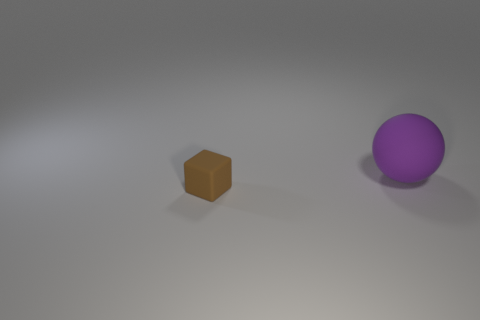
\includegraphics[width=\linewidth]{figures/CLEVR_DALE-TWO_example.png}}
  \caption{An example from the Dale-2 dataset}
  \label{fig:clevr-dale-2}
\end{figure}

In Figure \ref*{fig:clevr-dale-2}, the small red cube is the target object. Since all attributes except for the size are shared with the distractor, all three attributes are necessary, to identify it following \citet{Dale1995}'s rules, namely the \emph{small red cube}.


\begin{figure}[h]
  \centering
  \frame{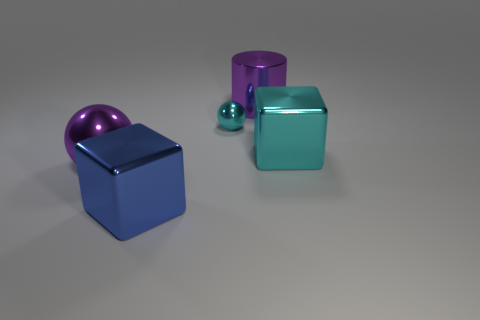
\includegraphics[width=\linewidth]{figures/CLEVR_DALE-FIVE_example.png}}
  \caption{An example from the Dale-5 dataset}
  \label{fig:clevr-dale-5}
\end{figure}
The target object in Figure \ref{fig:clevr-dale-5} is the purple cylinder. It shares the same colour and size with the purple sphere, the same size with the two cubes and no attribute with the turquoise sphere. It can be uniquely identified as the \emph{cylinder}.


\section{Setup of the language game}
\label{sec:setup-language-game}
%\begin{figure}
  \centering
  \frame{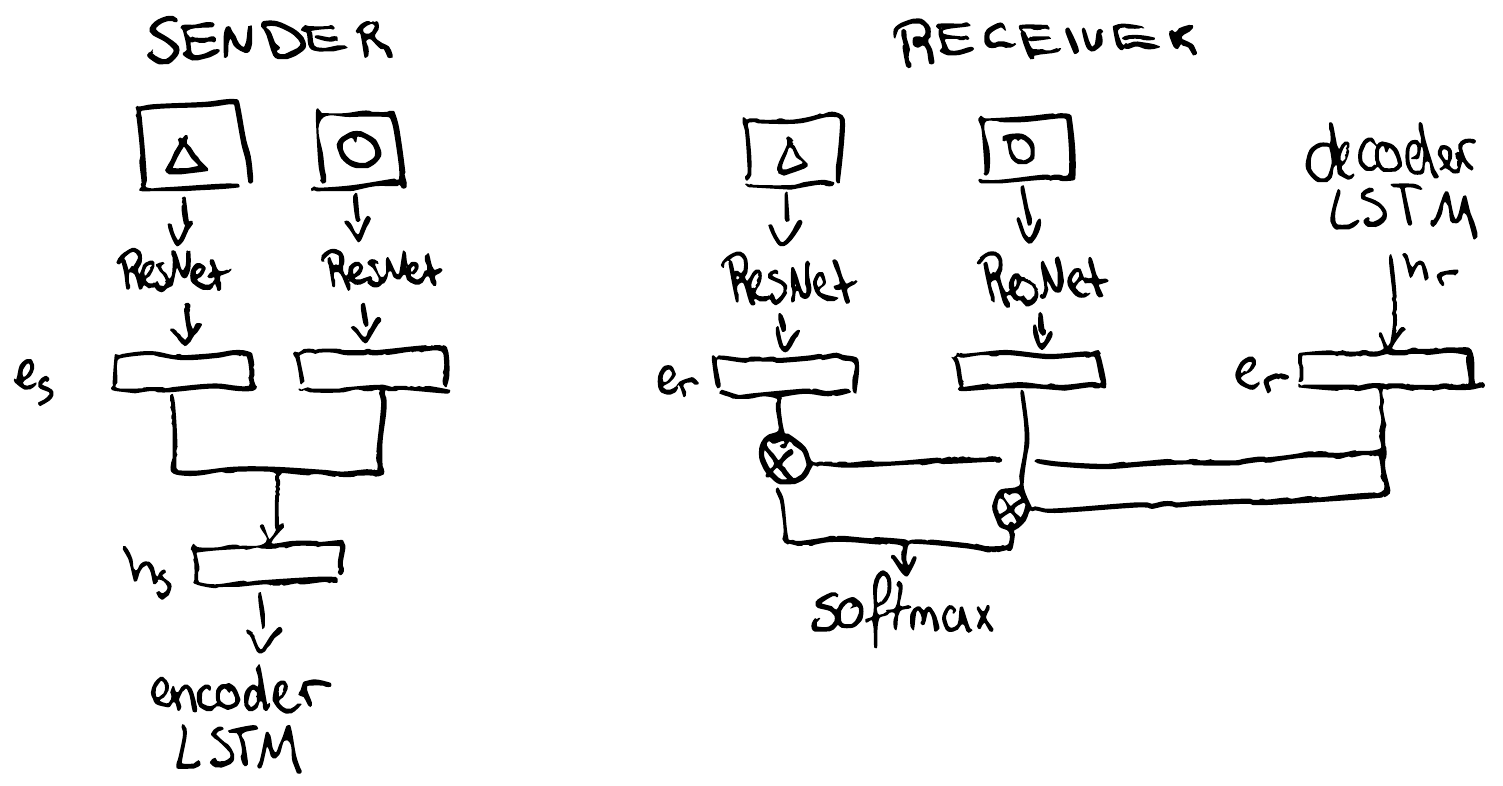
\includegraphics[width=\linewidth]{figures/architecture.png}}
  % \caption{Architectures of the sender and receiver}
%  \label{fig:architectures}
% \end{figure}

\end{document}
%%% Local Variables: 
%%% coding: utf-8
%%% mode: latex
%%% mode: flyspell
%%% ispell-local-dictionary: "british"
%%% TeX-engine: default
%%% TeX-master: t
%%% TeX-PDF-mode: t
%%% TeX-command-extra-options: "-shell-escape"
%%% End:
